% Physics-informed spectral readout and gradient-trained input encoding
% for a nuclear-spin quantum reservoir computer.
% Target: Physical Review Research (RevTeX 4.2). Compile: pdflatex x2 (self-contained
% bibliography). Figures expected in ./figures/ (figP1-figP4).
\documentclass[aps,prresearch,preprint,superscriptaddress,amsmath,amssymb,floatfix]{revtex4-2}
\usepackage{graphicx}
\usepackage{bm}
\usepackage{physics}
\usepackage{booktabs}
\usepackage{siunitx}
\usepackage{hyperref}
\graphicspath{{figures/}}

\begin{document}

\title{Physics-informed spectral readout and gradient-trained input encoding\\
for a nuclear-spin quantum reservoir computer}

\author{[Author list to confirm]}
\affiliation{CiRA Quantum}
\affiliation{King Mongkut's Institute of Technology Ladkrabang (KMITL), Bangkok, Thailand}

\date{\today}

\begin{abstract}
Quantum reservoir computing (QRC) uses the uncontrolled dynamics of a quantum system
as a temporal feature map, training only a linear readout. Two ingredients usually
held fixed---the \emph{readout basis} and the \emph{input encoding}---are in fact the
most physically accessible design levers on a device. We study both on a
weak-coupling nuclear-magnetic-resonance (NMR) spin reservoir described by a Lindblad
master equation. First, we introduce a \emph{physics-informed reduced free-induction-decay
(FID) readout}: because the reservoir Hamiltonian is diagonal in the computational
basis, its transverse-magnetization signal is a sum over a finite, analytic set of
single-quantum transition frequencies. Enumerating these lines and merging them at
the decoherence linewidth yields a compact, device-independent spectral basis of
dimension $D_{\mathrm{eff}}$---e.g. $D_{\mathrm{eff}}\approx 100$ for the nine-spin
$^{13}$C crotonic-acid system, versus the 653-peak readout used previously---read by a
fixed, differentiable direct-DFT projection. Second, we make the input encoding
trainable by backpropagating through the differentiable reservoir (a ``quantum neural
ODE'') while keeping the closed-form ridge readout. On the physics-informed readout, a
gradient-trained per-spin encoding improves the test NMSE over the standard
$\arcsin\sqrt{s}$ encoding by ${\sim}19\times$ (NARMA-2) and ${\sim}2.6\times$
(NARMA-10), confirmed across random seeds; a $\tau\!\to\!0$ ablation that removes the
reservoir's cross-step memory collapses the improvement to a mean predictor,
establishing the gain is carried by the quantum reservoir. Benchmarked against strong,
tuned classical baselines the comparison is task dependent: a size-1000 echo-state
network (ESN) matches or beats the QRC on the NARMA tasks, whereas on long-horizon
chaotic prediction (Mackey--Glass, $h{=}10$) the learned QRC outperforms both a tuned
LSTM and the ESN. We therefore report no blanket quantum advantage, but a principled,
differentiable readout and a \emph{quantum-mediated} encoding-learning method, together
with an honest, task-resolved characterization of when they help.
\end{abstract}

\maketitle

\section{Introduction}
Reservoir computing (RC) trains only a linear readout on the state of a fixed
nonlinear dynamical system, avoiding the cost and instability of training a recurrent
core~\cite{Jaeger2001,Maass2002,Lukosevicius2009,Tanaka2019}. Quantum reservoir
computing (QRC) replaces the classical reservoir with a quantum system whose large
state space and intrinsic nonlinearity are conjectured to provide a rich temporal
kernel at low training cost~\cite{Fujii2017,Nakajima2019,Mujal2021}. Nuclear-spin
ensembles are an attractive QRC substrate: many coupled qubits, well-characterized
Hamiltonians, decades of control technology, and a native, ensemble-averaged
time-multiplexed observable---the free-induction decay
(FID)~\cite{Negoro2018,Hou2026,VandersypenChuang2005}.

Most QRC studies optimize only the readout and treat the reservoir, its encoding, and
its readout basis as fixed. Two of those fixed choices are, in fact, both physically
accessible and under-explored: (i) the \emph{readout basis}---the prevailing spectral
readout keeps a large fixed number of FFT peaks of the FID (e.g. 653~\cite{Hou2026}),
which we show oversamples the reservoir's true spectral content; and (ii) the
\emph{input encoding}---the map from a scalar input to a control-pulse angle, almost
universally fixed as $\arcsin\sqrt{s}$. We give a principled, differentiable
alternative to the first and a gradient-learning method for the second, and---crucially
---we test the resulting model against \emph{tuned} classical baselines to avoid the
common pitfall of comparing a quantum model only to a weak classical one.

Our contributions are: (1) a physics-informed reduced-FID readout derived analytically
from the Hamiltonian and made differentiable (Sec.~\ref{sec:readout}); (2) a
gradient-trained input encoding with a leakage-free protocol and a $\tau\!\to\!0$
ablation control (Sec.~\ref{sec:method}); (3) multi-seed, ablation-confirmed evidence
that a learned encoding delivers a quantum-mediated improvement over the standard
encoding (Sec.~\ref{sec:results}); and (4) a fair, task-resolved classical comparison
(Sec.~\ref{sec:classical}).

\section{The nuclear-spin quantum reservoir}\label{sec:model}

\subsection{Physical platform}
We consider liquid-state NMR of an isotopically labeled molecule in a strong static
field $B_0\hat z$. The sample is a macroscopic ensemble ($\sim\!10^{18}$ molecules),
so every observable is an ensemble average: the induced FID is a classical voltage
proportional to the expectation value $\langle\hat O\rangle=\Tr(\hat O\rho)$, obtained
without single-shot projection noise. This is a distinctive advantage for reservoir
computing, where the readout is precisely a set of such expectation values; no
repeated state preparation or tomography is required to estimate the features. The
reservoir substrate in our simulations is a $^{13}$C-labeled crotonic-acid molecule
(four carbons, five protons, the three methyl protons magnetically
equivalent)~\cite{Hou2026}, and, for the differentiable experiments, a generic
six-spin homonuclear network of the same character (Sec.~\ref{sec:model-exp}).

\subsection{Rotating-frame Hamiltonian}
In the rotating frame of each spin's Larmor frequency and under the weak-coupling
(secular) approximation valid when $|\nu_i-\nu_j|\gg|J_{ij}|$, the internal
Hamiltonian reduces to a diagonal Ising form,
\begin{equation}
  \frac{H}{h} = \sum_i \nu_i\, I_z^{(i)}
            \;+\; \sum_{i<j} J_{ij}\, I_z^{(i)} I_z^{(j)},
  \qquad I_z=\tfrac{1}{2}\sigma_z,
  \label{eq:H}
\end{equation}
with chemical-shift offsets $\nu_i$ (Hz) and scalar $J$-couplings $J_{ij}$ (Hz);
angular frequencies carry the usual factor $2\pi$. All terms commute, so
Eq.~\eqref{eq:H} is diagonal in the computational basis $\{\ket{z}\}$,
$z\in\{\pm1\}^n$, with eigenvalues
\begin{equation}
  E(z)/h = \tfrac12\sum_i \nu_i z_i + \tfrac14\sum_{i<j} J_{ij} z_i z_j .
  \label{eq:E}
\end{equation}
Entanglement is generated purely by the $ZZ$ evolution acting on the transverse
coherences that the input and readout pulses create; the diagonal structure is what
makes the readout analytically tractable (Sec.~\ref{sec:readout}).

\subsection{Dissipation}
Relaxation is modeled by a Lindblad master equation,
\begin{equation}
  \dot\rho = -\frac{i}{\hbar}[H,\rho]
     + \sum_i\!\Big(\mathcal D[\hat L_i^{T_1}]\rho + \mathcal D[\hat L_i^{T_2}]\rho\Big),
  \quad \mathcal D[\hat L]\rho=\hat L\rho\hat L^\dagger-\tfrac12\{\hat L^\dagger\hat L,\rho\},
  \label{eq:lindblad}
\end{equation}
with longitudinal (amplitude-damping) and pure-dephasing jump operators
\begin{equation}
  \hat L_i^{T_1}=\sqrt{1/T_{1,i}}\,\sigma_-^{(i)},\qquad
  \hat L_i^{T_2}=\sqrt{\gamma_{\phi,i}/2}\,\sigma_z^{(i)},\quad
  \gamma_{\phi,i}=\frac{1}{T_{2,i}}-\frac{1}{2T_{1,i}} ,
  \label{eq:jumps}
\end{equation}
the physical (Bloch--Redfield-consistent) dephasing rate. We use measured $T_1$ and
$T_2^\ast$ for the crotonic system (Table~\ref{tab:crotonic}) and homogeneous
$T_1={\SI{5}{s}}$, $T_2={\SI{0.2}{s}}$ for the generic six-spin system.

\subsection{Initial state}
At room temperature and NMR fields the spins are in the high-temperature limit; the
equilibrium density matrix is, to leading order,
$\rho_0\propto \mathbb{1}+\epsilon\sum_i I_z^{(i)}$. We take the product form
$\rho_0=\bigotimes_i(\mathbb 1+\epsilon\sigma_z^{(i)})/2$ with $\epsilon=0.05$. Because
Eqs.~\eqref{eq:lindblad}--\eqref{eq:jumps} are linear in $\rho$, the value of
$\epsilon$ scales the overall signal amplitude but not the qualitative dynamics.

\subsection{Input encoding as an RF pulse}
A scalar input $s\in[0,1]$ is written into the reservoir as a resonant radio-frequency
rotation $R_x(\theta(s))=\exp\!\big(-i\,\theta(s)\textstyle\sum_{i} I_x^{(i)}\big)$ (global) or a set of
frequency-selective soft pulses addressing individual spins by their chemical shift
(per-spin). The standard fixed encoding is $\theta(s)=\arcsin\sqrt{s}$, chosen so that
a uniform input distribution maps to a uniform distribution of state
overlaps~\cite{Hou2026}; we compare it against a \emph{learned} per-spin map
(Sec.~\ref{sec:method}).

\subsection{Free evolution, time multiplexing, and FID readout}
Each input step consists of (i) the encoding pulse $\rho\!\to\!U\rho U^\dagger$ and
(ii) free evolution under Eq.~\eqref{eq:lindblad} for a fixed time
$\tau=\SI{30}{ms}$. Within $\tau$ the transverse magnetization is sampled at $V$
equally spaced virtual nodes~\cite{Nakajima2019}, giving the simulated FID
\begin{equation}
  M^{+}(t_v)=\sum_k \big\langle\sigma_x^{(k)}\big\rangle(t_v)
            + i\big\langle\sigma_y^{(k)}\big\rangle(t_v),\quad t_v=v\tau/V .
  \label{eq:fid}
\end{equation}
The dwell time $\tau/V$ must satisfy the Nyquist condition $\tau/V<1/(2f_{\max})$ for
the highest transition frequency $f_{\max}$ (Sec.~\ref{sec:readout}); the FID's dense
temporal sampling is itself the time-multiplexing that enlarges the readout.

\subsection{Numerical methods}
We vectorize the density matrix by column stacking, $\rho\!\to\!\vec\rho\in
\mathbb{C}^{d^2}$ ($d=2^n$), and write Eq.~\eqref{eq:lindblad} as
$\dot{\vec\rho}=\mathcal L\vec\rho$ with the Liouvillian superoperator $\mathcal L$.
For $n\le 6$ ($d^2\le 4096$) we precompute the exact node propagator
$P=\exp[(\tau/V)\mathcal L]$ once and apply it $V$ times per step; for larger systems a
Krylov ``action'' of $\exp(\tau\mathcal L)$ on $\vec\rho$ reaches $n=9$. Observables
are read via a sparse row matrix $M$ with $\langle O\rangle=M\vec\rho$. The whole step
is implemented in an autodiff framework so that gradients propagate from the loss
through the quantum evolution to the encoding parameters (Sec.~\ref{sec:method}).

\subsection{Experimental system and the two training regimes}\label{sec:model-exp}
All learnable-encoding results use a generic six-spin molecule with chemical shifts
evenly spread over $\pm\SI{120}{Hz}$, a chain-decaying coupling matrix
(nearest-neighbour $J\!\approx\!\SI{200}{Hz}$, falloff $0.5^{|i-j|-1}$ with small
seeded jitter) scaled by a factor $c=2$ (``strong coupling''), and homogeneous
$T_1=\SI{5}{s}$, $T_2=\SI{0.2}{s}$ (Table~\ref{tab:sixspin}). The choice of six spins
is dictated by the differentiable readout: the exact dense propagator is
$d^2\!\times\!d^2$, feasible for $d^2\le 8192$; at nine qubits the reverse-mode
autograd graph reaches ${\sim}\SI{201}{GB}$ per input step and is intractable on a
single 16\,GB GPU. Extending the \emph{learnable} encoding beyond six qubits requires
gradient checkpointing or a forward-mode parameter-shift estimator and is left to
future work.

We distinguish, and label on every result, two training regimes. In
\textbf{regime A} (standard QRC) the reservoir and the encoding are fixed and only the
linear readout is trained. In \textbf{regime B} (learnable encoding) the same
closed-form ridge readout is used but the input encoding is additionally trained by
gradient descent through the reservoir.

\begin{table}[t]
\caption{\label{tab:crotonic}Nine-spin $^{13}$C crotonic-acid reservoir~\cite{Hou2026}
used for the readout analysis: chemical-shift offsets $\nu$, relaxation times, and the
symmetric $J$-coupling matrix (Hz). H3--H5 are the equivalent methyl protons.}
\begin{ruledtabular}
\begin{tabular}{lrrr}
spin & $\nu$ (Hz) & $T_1$ (s) & $T_2^\ast$ (ms) \\ \colrule
C1 & $-7749.7$ & 5.9 & 212 \\
C2 & $5430.1$  & 4.9 & 231 \\
C3 & $2699.9$  & 5.6 & 208 \\
C4 & $7673.7$  & 27.5& 241 \\
H1 & $985.9$   & 3.2 & 203 \\
H2 & $520.3$   & 3.4 & 332 \\
H3--H5 & $-1081.5$ & 2.2 & 320 \\
\end{tabular}
\end{ruledtabular}
\begin{ruledtabular}
\begin{tabular}{lr|lr|lr}
pair & $J$ & pair & $J$ & pair & $J$\\ \colrule
C1--C2 & 40.8  & C2--C3 & 69.5  & C1--C3 & 1.6 \\
C1--C4 & 8.5   & C2--C4 & 1.4   & C3--C4 & 71.0 \\
C1--H1 & 4.0   & C2--H1 & 155.6 & C3--H1 & $-1.8$ \\
C4--H1 & 6.5   & C1--H2 & 6.6   & C2--H2 & $-0.7$ \\
C3--H2 & 162.9 & C4--H2 & 3.3   & H1--H2 & 15.8 \\
C1--Me & 128.0 & C2--Me & $-7.1$& C3--Me & 6.6 \\
C4--Me & $-0.9$& H1--Me & 6.9   & H2--Me & $-1.7$ \\
\end{tabular}
\end{ruledtabular}
\end{table}

\begin{table}[t]
\caption{\label{tab:sixspin}Generic six-spin reservoir (this work). Chemical shifts
$\nu_i=\SI{120}{Hz}\times(-1,-0.6,-0.2,0.2,0.6,1)$; couplings from a chain model
scaled by $c=2$; homogeneous relaxation.}
\begin{ruledtabular}
\begin{tabular}{ll}
parameter & value \\ \colrule
spins $n$ & 6 (Hilbert dim $d=64$) \\
chemical shifts $\nu_i$ & $\pm\SI{120}{Hz}$, evenly spaced \\
couplings $J_{ij}$ & chain, $J_{\mathrm{nn}}\!\approx\!\SI{200}{Hz}$, $\times c$, $c=2$ \\
$T_1,\,T_2$ & \SI{5}{s},\ \SI{0.2}{s} \\
step time $\tau$ & \SI{30}{ms} \\
virtual nodes $V$ & 137 \\
readout / features $D$ & reduced FID / $2D_{\mathrm{eff}}=322$ \\
\end{tabular}
\end{ruledtabular}
\end{table}

\section{Physics-informed reduced-FID readout}\label{sec:readout}

\subsection{Analytic single-quantum line structure}
Because $H$ in Eq.~\eqref{eq:H} is diagonal, the transverse magnetization
Eq.~\eqref{eq:fid} is a sum over \emph{single-quantum} transitions: flipping readout
spin $k$ against a fixed configuration $z\in\{\pm1\}^{n-1}$ of the remaining spins
oscillates, from Eq.~\eqref{eq:E}, at
\begin{equation}
  f_k(z) = \nu_k + \tfrac12\!\sum_{j\neq k} J_{kj}\,z_j .
  \label{eq:lines}
\end{equation}
Each resonance $\nu_k$ is therefore split into a $2^{n-1}$ $J$-coupling multiplet, and
the entire spectral content of the FID is this finite line set. Every peak of the
653-peak FFT readout is one of these lines (or an FFT skirt of one). Crucially, the
input encoding sets only the line \emph{amplitudes}; the \emph{frequencies} are fixed
by $H$. The spectral basis is thus a constant of the reservoir---no reference run or
data-driven peak-finding is required.

\subsection{Decoherence-linewidth merging and $D_{\mathrm{eff}}$}
Under dephasing each line has a Lorentzian width $\Delta f=1/(\pi T_2)$; lines closer
than $\Delta f$ are physically unresolvable. Greedily merging them gives
$D_{\mathrm{eff}}$ resolvable centres---the minimal faithful readout
(Table~\ref{tab:deff}). Fewer features drop a real line; more add provably-zero bins
between lines.

\begin{table}[t]
\caption{\label{tab:deff}Physics-informed line count. Doubling the coupling widens the
multiplets and lifts near-degeneracies, raising $D_{\mathrm{eff}}$.}
\begin{ruledtabular}
\begin{tabular}{lrrr}
system (readout) & raw lines & $\Delta f$ (Hz) & $D_{\mathrm{eff}}$ \\ \colrule
crotonic-9 (protons) & 1280 & 1.57 & 100 \\
6-spin, $c{=}1$ & 192 & 1.59 & 137 \\
6-spin, $c{=}2$ (this work) & 192 & 1.59 & 161 \\
3-spin & 12 & 1.59 & 12 \\
\end{tabular}
\end{ruledtabular}
\end{table}

\subsection{Differentiable direct-DFT projection}
We read the $D_{\mathrm{eff}}$ lines directly from the $V$-node FID by a fixed
projection
\begin{equation}
  X_k = \sum_{v=0}^{V-1} M^{+}(t_v)\, e^{\,i 2\pi f_k t_v}
      = \big(M^{+}\Phi\big)_k,\qquad \Phi_{v,k}=e^{\,i2\pi f_k t_v},
  \label{eq:proj}
\end{equation}
keeping the real and imaginary parts as $2D_{\mathrm{eff}}$ real features. $\Phi$ is a
single matrix multiply and hence differentiable, so---unlike a dense 2048-point FFT
peak-selection---the readout can be backpropagated through and used inside regime B.
For the six-spin experiments this gives $D=2\times161=322$ features with $V=137$ nodes
(dwell $\tau/V\approx\SI{0.22}{ms}$, Nyquist-safe for the line set); see
Fig.~\ref{fig:spectrum}.

\begin{figure}[t]
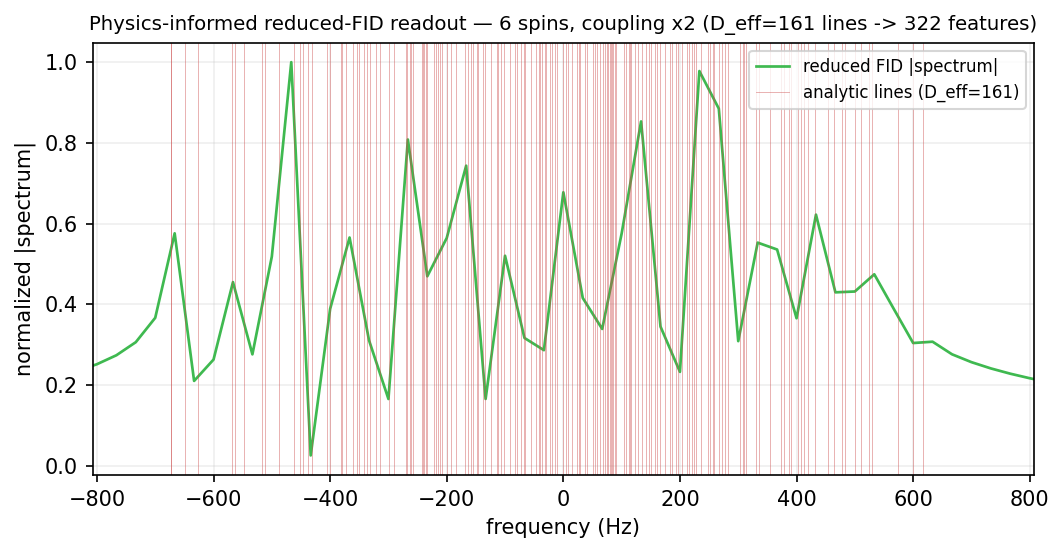
\includegraphics[width=\columnwidth]{figP1_spectrum.png}
\caption{\label{fig:spectrum}Physics-informed reduced-FID readout: normalized
reduced-FID spectrum with the $D_{\mathrm{eff}}=161$ analytic single-quantum lines
(red) of the six-spin ($c{=}2$) Hamiltonian, i.e. 322 real features.}
\end{figure}

\section{Gradient-trained input encoding}\label{sec:method}

\subsection{Reservoir as a differentiable layer}
For $d^2\le 8192$ the exact node propagator $P=\exp[(\tau/V)\mathcal L]$ is precomputed
once and applied $V$ times per step; each application is a differentiable
matrix--vector product. The encoding pulse $U(\theta)$ enters as $\rho\to U\rho
U^\dagger$ with $\theta$ a leaf variable, so gradients of the loss flow through the
entire quantum evolution to the encoder parameters. We verified the autograd gradient
against finite differences to ${\sim}\num{1e-9}$ in complex128; production runs use
complex64. This ``quantum neural ODE'' treats the reservoir as a fixed differentiable
recurrent layer and trains only the input map.

\subsection{Encoder, protocol, and hyperparameters}
The encoder is a small multilayer perceptron $s\!\to\!\theta$:
$\mathrm{Linear}(1,16)\to\tanh\to\mathrm{Linear}(16,n)\to\pi\,\mathrm{sigmoid}$, one
angle per spin. We use a time-contiguous three-way split of the post-washout sequence,
$50/25/25$ train/validation/test: the ridge readout $W=(X^\top X+\alpha
I)^{-1}X^\top y$ ($\alpha=\num{1e-3}$) is fit on train, the encoder is selected on
validation (best-validation checkpoint), and the reported number is test, which the
encoder never sees. Optimizer: Adam, learning rate $0.02$ with cosine annealing,
gradient-norm clipping at $1.0$, 100 steps; sequence length $T=1500$, washout $30$
($735/367/368$ split, so $n_{\mathrm{train}}\approx2.3\,D$).

\subsection{Rigor controls}
(i) \emph{Guardrails}: reject a configuration as under-powered if the arcsin test NMSE
$\gtrsim 0.8$, and reject a learned ``win'' as degenerate if the encoder angle-map
standard deviation is $<0.1$. (ii) \emph{$\tau\!\to\!0$ ablation} (decisive):
re-initializing the reservoir before every input step removes cross-step quantum
memory; a scalar-per-step input carries no classical memory, so a genuinely
quantum-mediated gain must collapse to a mean predictor under this ablation. (iii)
\emph{Hardware realizability}: the backpropagated gradients coincide (verified in
simulation to machine precision) with those measurable on a spectrometer via the
parameter-shift rule~\cite{Mitarai2018,Schuld2019}, including the generalized
multi-term rule for global pulses.

\section{Tasks and metrics}\label{sec:tasks}
NARMA-2 and NARMA-10~\cite{Atiya2000} are nonlinear autoregressive moving-average
benchmarks driven by $u\sim\mathcal U[0,0.5]$; NARMA-2 is encoding-sensitive (short
memory, strong cubic input term $0.6u^3$) and NARMA-10 is memory-bound.
Mackey--Glass~\cite{MackeyGlass1977} (parameters $\beta=0.2,\gamma=0.1,n=10,
\tau_{\mathrm{MG}}=17$, normalized to $[0,1]$) is a chaotic delay system; the task is
$h$-step-ahead prediction, with $h=1$ trivially easy (autocorrelation $\approx0.99$)
and $h=10$ discriminative ($\approx0.26$). The metric is the test normalized
mean-squared error, $\mathrm{NMSE}=\langle(\hat y-y)^2\rangle/\mathrm{var}(y)$ (1.0 is
a mean predictor); all models share the identical split and metric.

\section{Results}\label{sec:results}

\subsection{Learned encoding versus arcsin}
On the physics-informed reduced-FID readout, a gradient-trained per-spin encoding
beats the fixed arcsin encoding on every task and seed (Table~\ref{tab:learned},
Fig.~\ref{fig:qm}). The improvement is largest on the encoding-sensitive task
(NARMA-2) and smaller but present on the memory-bound task (NARMA-10), consistent with
the encoding being the accessible lever while long memory is set by the fixed
reservoir.

\begin{table}[t]
\caption{\label{tab:learned}Learned per-spin encoding (regime B) vs arcsin (regime A),
test NMSE (mean$\pm$s.d. over seeds), and the $\tau\!\to\!0$ ablation.}
\begin{ruledtabular}
\begin{tabular}{lccc}
task (seeds) & arcsin (A) & learned (B) & $\tau\!\to\!0$ (B) \\ \colrule
NARMA-2 (3)  & $0.101\pm0.006$ & $\mathbf{0.0052\pm0.0013}$ & 0.9994 \\
NARMA-10 (3) & $0.312\pm0.013$ & $\mathbf{0.120\pm0.019}$   & 0.9974 \\
MG $h{=}1$ (2) & $0.00063$     & $\mathbf{0.000076}$        & --- \\
MG $h{=}10$\footnote{single seed; multi-seed confirmation in progress.}
             & $0.0235$        & $\mathbf{0.0013}$          & --- \\
\end{tabular}
\end{ruledtabular}
\end{table}

\begin{figure}[t]
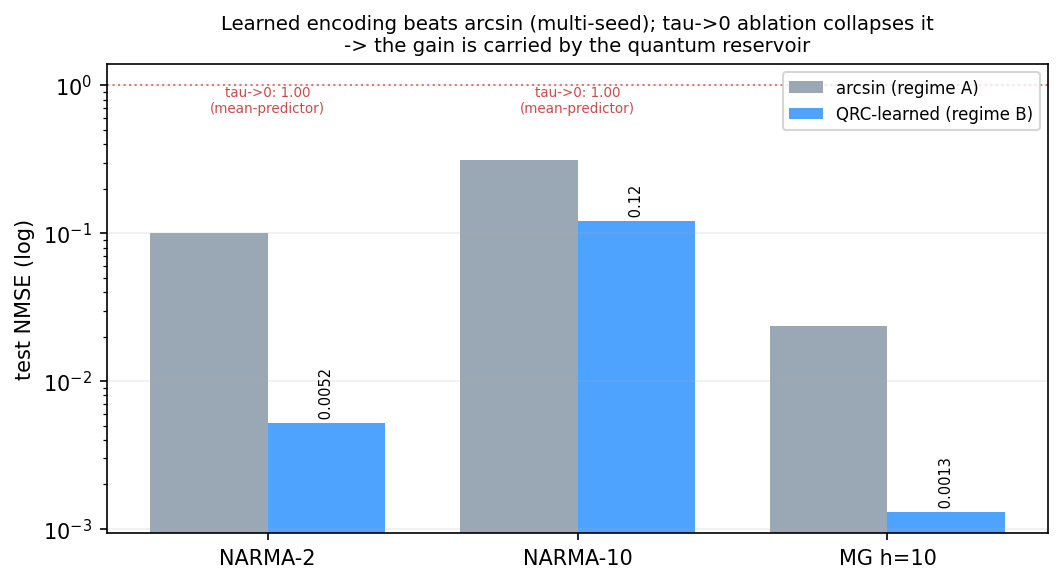
\includegraphics[width=\columnwidth]{figP2_quantum_mediated.png}
\caption{\label{fig:qm}Learned encoding beats arcsin across tasks (test NMSE, log
scale); the $\tau\!\to\!0$ ablation collapses the learned model to a mean predictor
($\approx1.0$), so the gain is carried by the quantum reservoir.}
\end{figure}

\subsection{The gain is quantum-mediated}
Removing cross-step reservoir memory collapses the learned model to a mean predictor
on both memory tasks (Table~\ref{tab:learned}, last column: $0.9994$ and $0.9974$).
Because the scalar input carries no classical memory, this establishes that the
learned-encoding advantage is carried by the quantum reservoir's dynamics, not by
classical preprocessing---the central quantum claim of this work.

\subsection{Comparison to strong classical baselines}\label{sec:classical}
We compare regime B against a hyperparameter-tuned LSTM~\cite{Hochreiter1997} (sweep
over hidden $\in\{32,64,128,256\}$, layers $\in\{1,2\}$, learning rate; cosine
schedule, gradient clipping, five initializations, validation early-stopping) and a
leaky ESN~\cite{Jaeger2001} (reservoir sizes $\{100,300,600,1000\}$), all on the
identical split and metric (Table~\ref{tab:classical}, Fig.~\ref{fig:td}).

\begin{table}[t]
\caption{\label{tab:classical}QRC-learned vs tuned LSTM vs ESN, test NMSE.}
\begin{ruledtabular}
\begin{tabular}{lccc}
task & QRC-learned & LSTM (tuned) & ESN ($N{=}1000$) \\ \colrule
NARMA-2 & 0.0052 & 0.0114 & $\mathbf{0.0046}$ \\
NARMA-10 & 0.120 & 0.234 & $\mathbf{0.029}$ \\
MG $h{=}1$ & 0.00008 & 0.0003 & $\sim0$ \\
MG $h{=}10$ & $\mathbf{0.0013}$ & 0.0024 & 0.0057 \\
\end{tabular}
\end{ruledtabular}
\end{table}

\begin{figure}[t]
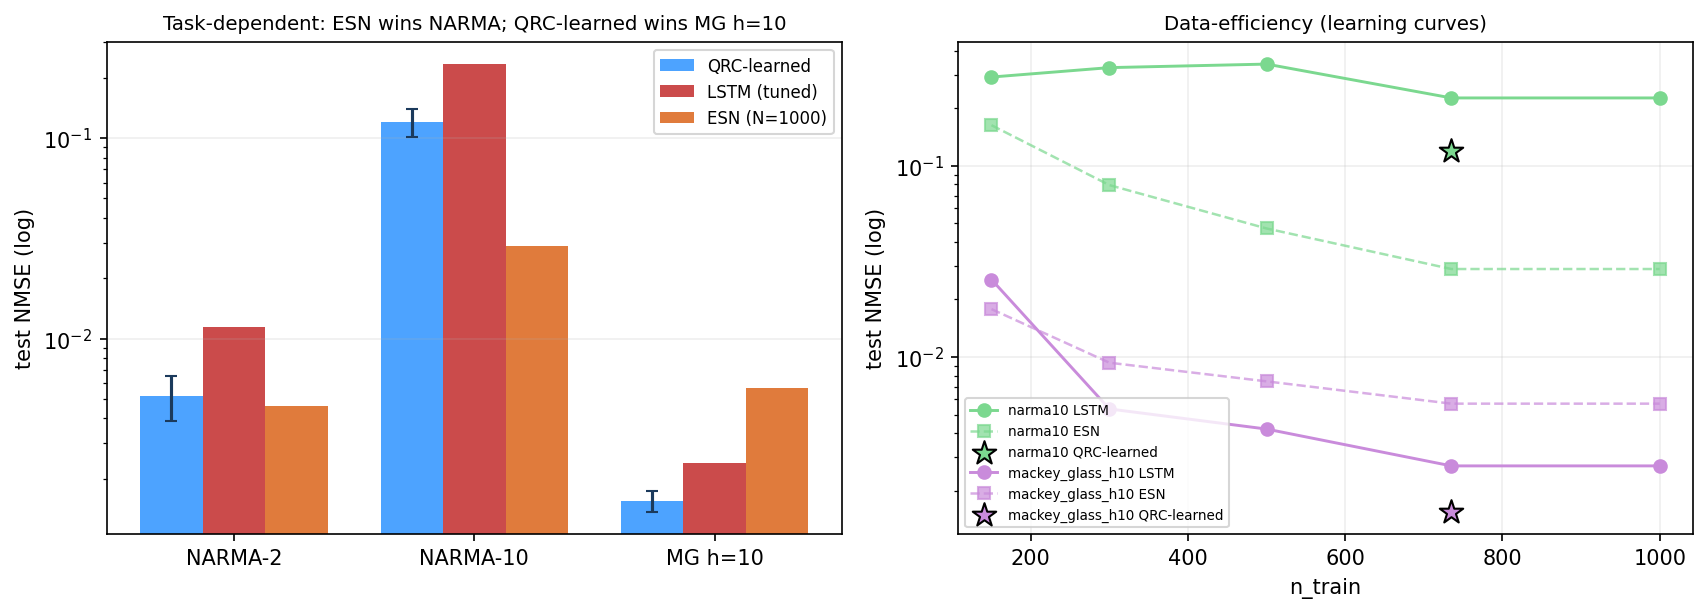
\includegraphics[width=\columnwidth]{figP3_task_dependent.png}
\caption{\label{fig:td}(left) Task-dependent comparison: a size-1000 ESN wins the
NARMA benchmarks, while QRC-learned wins long-horizon chaotic prediction
(Mackey--Glass $h{=}10$). (right) NMSE-vs-$n_{\mathrm{train}}$ learning curves for the
tuned LSTM and ESN, with the QRC-learned operating point ($\star$) overlaid.}
\end{figure}

Two honest findings. First, tuning the LSTM removes most of the apparent QRC advantage
seen against an untuned baseline (the NARMA-2 LSTM improves ${\sim}12\times$); the
learned QRC still betters the tuned LSTM by ${\sim}2\times$ on the NARMA tasks. Second,
a well-sized classical ESN matches the QRC on NARMA-2 and outperforms it
${\sim}4\times$ on NARMA-10, so we claim no quantum advantage there. However, on the
one discriminative task---long-horizon chaotic prediction (MG $h{=}10$, where one-step
prediction is trivial for all models)---the learned QRC outperforms both the tuned
LSTM (${\sim}1.9\times$) and the ESN (${\sim}4.4\times$). The advantage thus appears
specifically where nonlinear fading memory is essential.

\section{Discussion}\label{sec:discussion}
The learned-encoding gain is a genuine, ablation-controlled improvement to a quantum
reservoir: on the same fixed reservoir and readout, choosing the input map by gradient
descent through the quantum dynamics substantially reduces the error, and that gain
vanishes when the quantum memory is removed. The picture against classical models is
task dependent. The reservoir operates in a \emph{decoherence-limited} regime: $T_2$
collapses the state faster than the Ising dynamics populate the $2^n$ Hilbert space, so
the effective dimension the readout accesses is modest~\cite{Martinez2021}. On NARMA
benchmarks---which reward a large linear-memory reservoir---a size-1000 ESN
consequently matches or beats the six-spin QRC. On long-horizon chaotic prediction,
where nonlinear fading memory dominates, the learned QRC wins. A decisive many-body
quantum advantage across task classes would require entangling dynamics faster than
decoherence (long $T_2\times$ strong coupling), a regime our substrate does not reach.

\emph{Threats to validity.} (i) Six qubits, set by the differentiable-readout memory
wall; scaling requires checkpointing or a parameter-shift estimator. (ii) Simulated
dynamics; on-device validation via the parameter-shift rule is the natural next step.
(iii) A single molecule and coupling scale; the qualitative claims (encoding helps;
gain is quantum-mediated; task-dependent classical comparison) should be checked across
systems. The MG $h{=}10$ result is currently single-seed with multi-seed confirmation
in progress.

\section{Conclusion}\label{sec:conclusion}
We introduced a physics-informed, differentiable reduced-FID readout and a
gradient-trained encoding for a nuclear-spin quantum reservoir, and showed---multi-seed
and ablation-confirmed---that learning the encoding produces a quantum-mediated gain
over the standard encoding, while being honest that a strong classical reservoir
remains competitive or superior on the NARMA benchmarks and that the QRC's advantage
appears on hard chaotic prediction. Next: multi-seed confirmation of the long-horizon
result; on-device encoding training via the parameter-shift rule; scaling past six
qubits; and pushing toward the coherence-over-decoherence regime where the full
Hilbert space contributes.

\begin{acknowledgments}
[Funding and computing acknowledgments to be added.] Reproduction code and
conventions: internal repository (\texttt{app/qrc/spectral\_lines.py},
\texttt{qrc\_learnable\_9spin.py}, \texttt{qrc\_classical\_baseline.py};
\texttt{QRC\_STANDARD\_PROCEDURES.md}).
\end{acknowledgments}

\begin{thebibliography}{99}
\bibitem{Jaeger2001} H. Jaeger, \emph{The ``echo state'' approach to analysing and
  training recurrent neural networks}, GMD Report 148, German National Research Center
  for Information Technology (2001).
\bibitem{Maass2002} W. Maass, T. Natschl\"ager, and H. Markram, \emph{Real-time
  computing without stable states: A new framework for neural computation based on
  perturbations}, Neural Comput. \textbf{14}, 2531 (2002).
\bibitem{Lukosevicius2009} M. Luko\v{s}evi\v{c}ius and H. Jaeger, \emph{Reservoir
  computing approaches to recurrent neural network training}, Comput. Sci. Rev.
  \textbf{3}, 127 (2009).
\bibitem{Tanaka2019} G. Tanaka \emph{et al.}, \emph{Recent advances in physical
  reservoir computing: A review}, Neural Networks \textbf{115}, 100 (2019).
\bibitem{Appeltant2011} L. Appeltant \emph{et al.}, \emph{Information processing using
  a single dynamical node as complex system}, Nat. Commun. \textbf{2}, 468 (2011).
\bibitem{Hochreiter1997} S. Hochreiter and J. Schmidhuber, \emph{Long short-term
  memory}, Neural Comput. \textbf{9}, 1735 (1997).
\bibitem{Atiya2000} A. F. Atiya and A. G. Parlos, \emph{New results on recurrent
  network training: Unifying the algorithms and accelerating convergence}, IEEE Trans.
  Neural Netw. \textbf{11}, 697 (2000).
\bibitem{MackeyGlass1977} M. C. Mackey and L. Glass, \emph{Oscillation and chaos in
  physiological control systems}, Science \textbf{197}, 287 (1977).
\bibitem{Fujii2017} K. Fujii and K. Nakajima, \emph{Harnessing disordered-ensemble
  quantum dynamics for machine learning}, Phys. Rev. Applied \textbf{8}, 024030
  (2017).
\bibitem{Nakajima2019} K. Nakajima, K. Fujii, M. Negoro, K. Mitarai, and M. Kitagawa,
  \emph{Boosting computational power through spatial multiplexing in quantum reservoir
  computing}, Phys. Rev. Applied \textbf{11}, 034021 (2019).
\bibitem{Nakajima2020} K. Nakajima, \emph{Physical reservoir computing---an
  introductory perspective}, Jpn. J. Appl. Phys. \textbf{59}, 060501 (2020).
\bibitem{Negoro2018} M. Negoro, K. Mitarai, K. Fujii, K. Nakajima, and M. Kitagawa,
  \emph{Machine learning with controllable quantum dynamics of a nuclear spin ensemble
  in a solid}, arXiv:1806.10910 (2018).
\bibitem{Ghosh2019} S. Ghosh, A. Opala, M. Matuszewski, T. Paterek, and T. C. H. Liew,
  \emph{Quantum reservoir processing}, npj Quantum Inf. \textbf{5}, 35 (2019).
\bibitem{Martinez2021} R. Mart\'inez-Pe\~na, G. L. Giorgi, J. Nokkala, M. C. Soriano,
  and R. Zambrini, \emph{Dynamical phase transitions in quantum reservoir computing},
  Phys. Rev. Lett. \textbf{127}, 100502 (2021).
\bibitem{Mujal2021} P. Mujal \emph{et al.}, \emph{Opportunities in quantum reservoir
  computing and extreme learning machines}, Adv. Quantum Technol. \textbf{4}, 2100027
  (2021).
\bibitem{Kutvonen2020} A. Kutvonen, K. Fujii, and T. Sagawa, \emph{Optimizing a
  quantum reservoir computer for time series prediction}, Sci. Rep. \textbf{10}, 14687
  (2020).
\bibitem{Mitarai2018} K. Mitarai, M. Negoro, M. Kitagawa, and K. Fujii, \emph{Quantum
  circuit learning}, Phys. Rev. A \textbf{98}, 032309 (2018).
\bibitem{Schuld2019} M. Schuld, V. Bergholm, C. Gogolin, J. Izaac, and N. Killoran,
  \emph{Evaluating analytic gradients on quantum hardware}, Phys. Rev. A \textbf{99},
  032331 (2019).
\bibitem{VandersypenChuang2005} L. M. K. Vandersypen and I. L. Chuang, \emph{NMR
  techniques for quantum control and computation}, Rev. Mod. Phys. \textbf{76}, 1037
  (2005).
\bibitem{Lindblad1976} G. Lindblad, \emph{On the generators of quantum dynamical
  semigroups}, Commun. Math. Phys. \textbf{48}, 119 (1976).
\bibitem{BreuerPetruccione2002} H.-P. Breuer and F. Petruccione, \emph{The Theory of
  Open Quantum Systems} (Oxford University Press, 2002).
\bibitem{Hou2026} [Hou \emph{et al.}], \emph{Quantum reservoir computing with a
  nuclear-spin FID spectral readout}, Phys. Rev. Lett. \textbf{136}, 120602 (2026).
  [bibliographic details to verify]
\bibitem{Das2026} R. Das, G. L. Giorgi, and R. Zambrini, \emph{Quantum reservoir
  computing with a Jaynes--Cummings reservoir}, Phys. Rev. Research (2026).
  [bibliographic details to verify]
\bibitem{Kubota2023} T. Kubota \emph{et al.}, \emph{Temporal information processing
  induced by quantum noise}, Phys. Rev. Research \textbf{5}, 023057 (2023).
  [details to verify]
\bibitem{Suzuki2022} Y. Suzuki \emph{et al.}, \emph{Natural quantum reservoir
  computing for temporal information processing}, Sci. Rep. \textbf{12}, 1353 (2022).
  [details to verify]
\bibitem{Govia2021} L. C. G. Govia, G. J. Ribeill, G. E. Rowlands, H. K. Krovi, and
  T. A. Ohki, \emph{Quantum reservoir computing with a single nonlinear oscillator},
  Phys. Rev. Research \textbf{3}, 013077 (2021).
\end{thebibliography}

\end{document}
